\documentclass[a4paper,oneside,titlepage,10pt]{article}
\usepackage{xltxtra}
\usepackage{xgreek}
\setmainfont[Mapping=tex-text]{Calibri.ttf} %Courier New for programing
\usepackage{amsfonts}
\usepackage{listings}

\usepackage[table,xcdraw]{xcolor}

%\setmainfont[Mapping=tex-text]{Helvetica}
\setmainfont[Mapping=tex-text]{Calibri.ttf}
\setmainfont[
 BoldFont={CALIBRIB.TTF}, 
 ItalicFont={CALIBRII.TTF},
 BoldItalicFont={CALIBRIZ.TTF}
 ]{Calibri.ttf}

\usepackage[margin=1in]{geometry}

\usepackage[hidelinks]{hyperref}

\usepackage{enumitem}


%\usepackage[LGR]{fontenc}

%\renewcommand{\familydefault}{\sfdefault}



\usepackage{graphicx,wrapfig}
\graphicspath{ {images/} }

%\usepackage[usenames, dvipsnames]{color}
%\definecolor{mygray}{gray}{0.6}



\definecolor{calpolypomonagreen}{rgb}{0.07, 0.53, 0.03}


\usepackage{listings}

\lstdefinelanguage{diff}{
  morecomment=[f][\color{blue}]{@@},     % group identifier
  morecomment=[f][\color{red}]-,         % deleted lines 
  morecomment=[f][\color{calpolypomonagreen}]+,       % added lines
  morecomment=[f][\color{magenta}]{---}, % Diff header lines (must appear after +,-)
  morecomment=[f][\color{magenta}]{+++},
}

\lstdefinelanguage{diffrrr}{
  sensitive=true,
  % diff command line
  morecomment=[f][\color{gray}][0]{diff},
  % commit identifiers for git diff
  morecomment=[f][\color{gray}][0]{index},
  % hunk location/line numbers for unified format
  morecomment=[f][\color{blue}][0]{@@},
  % hunk location/line numbers for context format
  morecomment=[f][\color{magenta}][0]{***},
  % changed line for context format
  morecomment=[f][\color{violet}][0]{!},
  % deleted lines for unified format
  morecomment=[f][\color{red!60!black}][0]-,
  % added lines for unified format
  morecomment=[f][\color{green!60!black}][0]+,
  % file name and time stamp old file
  morecomment=[f][\color{magenta}][0]{---},
  % file name and time stamp new file
  morecomment=[f][\color{magenta}][0]{+++},
  % Binary files ... differ
  morecomment=[f][\color{gray}][0]{Binary},
  % Only in ...: file.txt
  morecomment=[f][\color{gray}][0]{Only},
  % old mode ...
  morecomment=[f][\color{gray}][0]{old},
  % new mode ...
  morecomment=[f][\color{gray}][0]{new},
  % rename from/to ...
  morecomment=[f][\color{gray}][0]{rename},
  % similarity index ...%
  morecomment=[f][\color{gray}][0]{similarity},
  % deleted file mode ...%
  morecomment=[f][\color{gray}][0]{deleted},
  % hunk separator for context format
  morecomment=[f][\color{magenta}][0]{***************},
  % deleted lines for normal format
  morecomment=[f][\color{red!60!black}][0]<,
  % added lines for normal format
  morecomment=[f][\color{green!60!black}][0]>,
  % line number specifier for normal format
  morecomment=[f][\color{blue}][0]{0},
  % line number specifier for normal format
  morecomment=[f][\color{blue}][0]{1},
  % line number specifier for normal format
  morecomment=[f][\color{blue}][0]{2},
  % line number specifier for normal format
  morecomment=[f][\color{blue}][0]{3},
  % line number specifier for normal format
  morecomment=[f][\color{blue}][0]{4},
  % line number specifier for normal format
  morecomment=[f][\color{blue}][0]{5},
  % line number specifier for normal format
  morecomment=[f][\color{blue}][0]{6},
  % line number specifier for normal format
  morecomment=[f][\color{blue}][0]{7},
  % line number specifier for normal format
  morecomment=[f][\color{blue}][0]{8},
  % line number specifier for normal format
  morecomment=[f][\color{blue}][0]{9},
}[comments]

\definecolor{verbgray}{gray}{0.93}




\lstdefinestyle{myCustomMatlabStyle}{
  language=diff,
  backgroundcolor=\color{verbgray},
  stepnumber=1,
  numbersep=10pt,
  tabsize=4,
  showspaces=false,
  keepspaces=true,
  showstringspaces=false,
  frame=single,
  framerule=0pt,
  columns=fullflexible,
  basicstyle=\ttfamily\footnotesize
}

\lstdefinestyle{myCustomCStyle}{
  language=C,
  backgroundcolor=\color{verbgray},
  stepnumber=1,
  numbersep=10pt,
  tabsize=4,
  showspaces=false,
  showstringspaces=false,
  frame=single,
  framerule=0pt,
  columns=fullflexible,
  basicstyle=\ttfamily\footnotesize
}

\lstdefinestyle{CStyle}{
    backgroundcolor=\color{verbgray},   
    commentstyle=\color{green},
    keywordstyle=\color{magenta},
    numberstyle=\tiny\color{gray}\ttfamily,
    numbers=left,
    stringstyle=\color{purple},
    basicstyle=\ttfamily\small,
    breakatwhitespace=false,         
    breaklines=true,                 
    captionpos=b,                    
    keepspaces=true,                 
    showspaces=false,                
    showstringspaces=false,
    showtabs=false,                  
    tabsize=4,
    columns=fullflexible,
                keywordstyle=\color{blue}\ttfamily,
                stringstyle=\color{red}\ttfamily,
                commentstyle=\color{calpolypomonagreen}\ttfamily,
                morecomment=[l][\color{magenta}]{\#}
    language=C
}

\lstdefinestyle{bash}{
    backgroundcolor=\color{black},   
    commentstyle=\color{white},
    keywordstyle=\color{white},
    stringstyle=\color{white},
    basicstyle=\ttfamily\color{white}\small,
    breakatwhitespace=false,         
    breaklines=true,                 
    %captionpos=b,                    
    keepspaces=true,                 
    showspaces=false,                
    showstringspaces=false,
    showtabs=false,                  
    tabsize=4,
    linewidth=15cm,
    language=C
    %columns=fullflexible,
}



\begin{document}

\begin{center}
    \thispagestyle{empty}
    
\includegraphics[scale=0.9]{logo.jpg}
    
    \vspace{0.5cm}
    
    \textsc{\large Πολυτεχνική Σχολή \\ Τμήμα Μηχανικών Ηλεκτρονικών Υπολογιστών \& Πληροφορικής}
    
    \vspace{0.75cm}
    
    {\huge \noindent\textbf{Παράλληλη Επεξεργασία}
    \vspace{0.1cm}
\\ {\Large \textbf{Εργασία Εαρινού Εξαμήνου 2017-2018}}}

\vspace{1cm}
    
    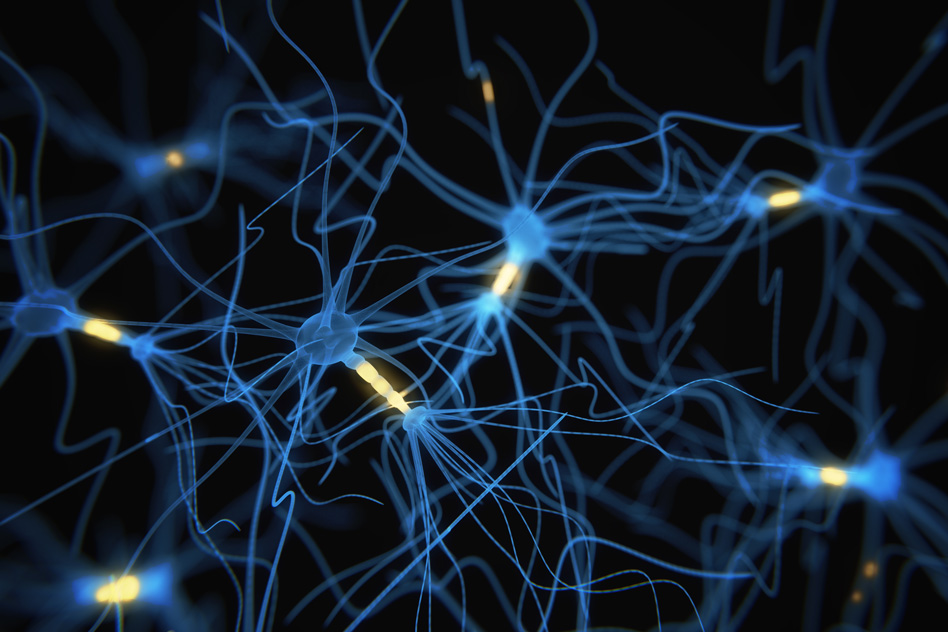
\includegraphics[scale=0.4]{neur.jpg}
    
%     \begin{center}
% {\par\bigskip
% \begin{minipage}[b]{0.33333\textwidth}
% \centering
% Σταυρούλα Δρίτσα, 6040 \par
% \texttt{dritsa@ceid.upatras.gr}
% \end{minipage}%
% \begin{minipage}[b]{0.33333\textwidth}
% \centering
% Νικόλαος Ζαχαρόπουλος, 6048 \par
% \texttt{zachar@ceid.upatras.gr}
% \end{minipage}%
% \begin{minipage}[b]{0.33333\textwidth}
% \centering
% Δαμιανός Ντούμη - Σιγάλας, 6157 \par
% \texttt{nsigalas@ceid.upatras.gr}
% \end{minipage}
% \end{center}

\vspace{1.5cm}

Σταυρούλα Δρίτσα, 6040 \par
\texttt{dritsa@ceid.upatras.gr}

\vspace{0.5cm}

Νικόλαος Ζαχαρόπουλος, 6048 \par
\texttt{zachar@ceid.upatras.gr}

\vspace{0.5cm}

Δαμιανός Ντούμη - Σιγάλας, 6157 \par
\texttt{nsigalas@ceid.upatras.gr}


\end{center}

% \newpage
% \begin{center}{\textsc{Πανεπιστήμιο Πατρών - Πολυτεχνική Σχολή} \\ \textsc{Τμήμα Μηχανικών Ηλεκτρονικών Υπολογιστών \& Πληροφορικής} }	
% \end{center}

% {\Large \noindent\textbf{Παράλληλη Επεξεργασία}
% \hfill {\large \textbf{Εργασία Εαρινού Εξαμήνου 2017-2018}}}

% \vspace{1cm}

% \noindent \textbf{Εργασία Φοιτητών:}
% \vspace{-0.4cm}
% \begin{center}
% {\par\bigskip
% \begin{minipage}[b]{0.33333\textwidth}
% \centering
% Σταυρούλα Δρίτσα, 6040 \par
% \texttt{dritsa@ceid.upatras.gr}
% \end{minipage}%
% \begin{minipage}[b]{0.33333\textwidth}
% \centering
% Νικόλαος Ζαχαρόπουλος, 6048 \par
% \texttt{zachar@ceid.upatras.gr}
% \end{minipage}%
% \begin{minipage}[b]{0.33333\textwidth}
% \centering
% Δαμιανός Ντούμη - Σιγάλας, 6157 \par
% \texttt{nsigalas@ceid.upatras.gr}
% \end{minipage}
% \end{center}


\lstset{basicstyle=\large,style=myCustomMatlabStyle}


\setlength{\parskip}{10pt}%

\section*{Ακολουθιακό Πρόγραμμα}

\section*{Ζητούμενο 1Α - Βελτιστοποίηση Αντιγραφών}

Στον κώδικα που μας δίνεται παρατηρούμε ότι στο τέλος κάθε επανάληψης η νέα τιμή δυναμικού του κάθε νευρώνα (διάνυσμα uplus), αντιγράφεται στην προηγούμενη (διάνυσμα u). Αυτή η διαδικασία εισάγει έναν μεγάλο αριθμό επαναλήψεων ο οποίος μπορεί να αποφευχθεί εναλλάσσοντας την τιμή των δεικτών των διανυσμάτων uplus και u μεταξύ τους, όπως φαίνεται στον κώδικα παρακάτω. 

\lstinputlisting[language=diff]{code/1a.patch}

\noindent Τα αποτελέσματα που παίρνουμε από την εκτέλεση του προγράμματος μετά τις αλλαγές έχουν ως εξής:

\setcounter{page}{1}


\begin{table}[!h]
	\centering
	\begin{tabular}{|c|c|c|c|c|}
		\hline
		\multicolumn{5}{|c|}{\cellcolor[HTML]{EFEFEF}\texttt{\textbf{gcc -O3 -Wall -Wextra lif1d.c}}}                       \\ \hline
		\textbf{n} & \textbf{r} & \textbf{Calculation Time} & \textbf{I/O Time} & \textbf{Execution Time} \\ \hline
		1000       & 350        & 142,934061                & 0,010088          & 142,944149              \\ \hline
		2000       & 700        &                           &                   & 0,000000                \\ \hline
		3000       & 1000       &                           &                   & 0,000000                \\ \hline
		4000       & 1300       &                           &                   & 0,000000                \\ \hline
		5000       & 1600       &                           &                   & 0,000000                \\ \hline
	\end{tabular}
\end{table}

\begin{table}[!h]
	\centering
	\begin{tabular}{|c|c|c|c|c|}
		\hline
		\multicolumn{5}{|c|}{\texttt{\textbf{gcc -O3 -Wall -Wextra lif1d.c}}}                                              \\ \hline
		\textbf{n} & \textbf{r} & \textbf{Calculation Time} & \textbf{I/O Time} & \textbf{Execution Time} \\ \hline
		1000       & 350        & 142,934061                & 0,010088          & 142,944149              \\ \hline
		2000       & 700        &                           &                   & 0,000000                \\ \hline
		3000       & 1000       &                           &                   & 0,000000                \\ \hline
		4000       & 1300       &                           &                   & 0,000000                \\ \hline
		5000       & 1600       &                           &                   & 0,000000                \\ \hline
	\end{tabular}
\end{table}

\newpage

\section*{Ζητούμενο 1B - Αναδιοργάνωση Υπολογισμών }

\noindent Η σχέση που μας δίνει το νέο δυναμικό του νευρώνα i την χρονική στιγμή t + Δt είναι η εξής:

$$
u_{i}(t+\Delta t) = u_{i}(t) + \Delta t \cdot \Bigg(\mu - u_{i}(t) + \frac{1}{N_{c}} \sum_{j \in \{N_{i}\}}^{N_{c}}\sigma_{ij} \cdot [u_{j}(t) - u_{i}(t)]\Bigg)
$$

\noindent Στην σχέση αυτή θα προσπαθήσουμε να αναδιοργανώσουμε τους υπολογισμούς που γίνονται στο άθροισμα:

$$
\sum_{j \in \{N_{i}\}}^{N_{c}}\sigma_{ij} \cdot [u_{j}(t) - u_{i}(t)] =
\sum_{j \in \{N_{i}\}}^{N_{c}}\sigma_{ij} u_{j}(t)\ \    - \sum_{j \in \{N_{i}\}}^{N_{c}}\sigma_{ij} u_{i}(t) = 
\sum_{j \in \{N_{i}\}}^{N_{c}}\sigma_{ij} u_{j}(t)\ \    - u_{i}(t)\sum_{j \in \{N_{i}\}}^{N_{c}}\sigma_{ij} 
$$

\noindent Στο δεύτερο άθροισμα που έχει προκύψει παρατηρούμε ότι ο όρος $u_{i}(t)$ είναι ανεξάρτητος του j και επομένως μπορεί να βγει έξω από αυτό. Συνεπώς για κάθε j χρησιμοποιείται το άθροισμα της i-οστής γραμμής του μητρώου σ. Ο όρος αυτός είναι σταθερός και ανεξάρτητος από κάθε επανάληψη της προσομοίωσης μας. Γι' αυτόν τον τον λόγο και με σκοπό να εξοικονομήσουμε περιττούς υπολογισμούς δημιουργούμε πριν την έναρξη της προσομοίωσης ένα διάνυσμα \texttt{sigma\_vector} μήκους n στο οποίο υπολογίζουμε σε κάθε θέση το άθροισμα της αντίστοιχης γραμμής του μητρώου. Έπειτα όπου χρειάζεται αντί να υπολογίζουμε εκ νέου την τιμή θα ανατρέχουμε σε αυτό. Ουσιαστικά μας ενδιαφέρει πως κάθε νευρώνας i επηρεάζεται από το δυναμικό των j γειτόνων του, με την μορφή του διανύσματος να είναι η παρακάτω: 

\begin{table}[!h]
	\centering
	\begin{tabular}{|l|l|l|l|l|}
		\hline
		$\sum \sigma_{1j}$ & $\sum \sigma_{2j}$ & $\sum \sigma_{3j}$ & ... & $\sum \sigma_{nj}$ \\ \hline
	\end{tabular}
\end{table}

\noindent Οι παραπάνω αλλαγές στον κώδικα συνοψίζονται ως εξής:

\lstinputlisting[language=diff]{code/1b.patch}

\noindent Τα αποτελέσματα που παίρνουμε από την εκτέλεση του προγράμματος μετά τις αλλαγές έχουν ως εξής:

\begin{table}[!h]
	\centering
	\begin{tabular}{|c|c|c|c|c|}
		\hline
		\multicolumn{5}{|c|}{\cellcolor[HTML]{EFEFEF}\texttt{\textbf{gcc -O3 -Wall -Wextra lif1d.c}}}                       \\ \hline
		\textbf{n} & \textbf{r} & \textbf{Calculation Time} & \textbf{I/O Time} & \textbf{Execution Time} \\ \hline
		1000       & 350        & 142,934061                & 0,010088          & 142,944149              \\ \hline
		2000       & 700        &                           &                   & 0,000000                \\ \hline
		3000       & 1000       &                           &                   & 0,000000                \\ \hline
		4000       & 1300       &                           &                   & 0,000000                \\ \hline
		5000       & 1600       &                           &                   & 0,000000                \\ \hline
	\end{tabular}
\end{table}

\begin{table}[!h]
	\centering
	\begin{tabular}{|c|c|c|c|c|}
		\hline
		\multicolumn{5}{|c|}{\texttt{\textbf{gcc -O3 -Wall -Wextra lif1d.c}}}                                              \\ \hline
		\textbf{n} & \textbf{r} & \textbf{Calculation Time} & \textbf{I/O Time} & \textbf{Execution Time} \\ \hline
		1000       & 350        & 142,934061                & 0,010088          & 142,944149              \\ \hline
		2000       & 700        &                           &                   & 0,000000                \\ \hline
		3000       & 1000       &                           &                   & 0,000000                \\ \hline
		4000       & 1300       &                           &                   & 0,000000                \\ \hline
		5000       & 1600       &                           &                   & 0,000000                \\ \hline
	\end{tabular}
\end{table}

\newpage
\section*{Ζητούμενο 1C - Χρήση βιβλιοθήκης BLAS }

\noindent Στο προηγούμενο ερώτημα ασχοληθήκαμε με την βελτιστοποίηση του δεύτερου αθροίσματος όπως προέκυψε μετά την αναδιοργάνωση των υπολογισμών. Τώρα θα προσπαθήσουμε να βελτιστοποιήσουμε το πρώτο άθροισμα κάνοντας χρήση της βιβλιοθήκης συναρτήσεων BLAS. Το άθροισμα αυτό έχει την μορφή:

$$
\sum_{j \in \{N_{i}\}}^{N_{c}}\sigma_{ij} u_{j}(t)
$$ 

\noindent Παρατηρούμε ότι για κάθε νευρώνα i υπολογίζουμε πως επηρεάζεται από το δυναμικό του νευρώνα j. Η πράξη αυτή αντιστοιχεί με τον πολλαπλασιασμό του μητρώου σ επί διάνυσμα u. Θα χρησιμοποιήσουμε την βιβλιοθήκη BLAS η οποία παρέχει συναρτήσεις για τον υπολογισμό τέτοιου είδους πράξεων με πολύ πιο αποδοτικό τρόπο. Συγκεκριμένα θα χρειαστούμε την συνάρτηση dgemv η οποία εκτελεί την παρακάτω σχέση για double ακρίβειας δεδομένα:

$$
y = \alpha A x + \beta y
$$

\noindent όπου Α είναι το μητρώο εισόδου διαστάσεων NxM, x το διάνυσμα, α και β βαθμωτοί και y το τελικό αποτέλεσμα. Επομένως η κλήση της συνάρτησης για τα δικά μας δεδομένα θα έχει την μορφή:

\texttt{
cblas\_dgemv(CblasRowMajor, CblasNoTrans, n, n, 1, sigma, n, u, 1, 0, mysum1, 1);
}

\noindent όπου:

\vspace{-0.5cm}

\begin{description}
	\item[CblasRowMajor] το μητρώο σ είναι δομημένο κατά γραμμές 
	\item[CblasNoTrans] δεν θέλουμε το ανάστροφο του μητρώου σ
	\item[n] η διάσταση Μ του μητρώου
	\item[n] η διάσταση Ν του μητρώου
	\item[1] η τιμή του βαθμωτού α
	\item[sigma] το μητρώο εισόδου
	\item[n] η διάσταση Μ του διανύσματος u (nx1)
	\item[u] το διάνυσμα
	\item[1] incX, το βήμα για τον εντοπισμό του επόμενου στοιχείου του διανύσματος
	\item[0] η τιμή του βαθμωτού β
	\item[mysum1] το διάνυσμα y στο οποίο αποθηκεύεται το αποτέλεσμα
	\item[1] incΥ, το βήμα για τον εντοπισμό του επόμενου στοιχείου του διανύσματος y
	
\end{description}

\noindent Συνολικά οι αλλαγές στον κώδικα είναι οι εξής:

\lstinputlisting[language=diff]{code/1c.patch}



% Lorem ipsum dolor sit amet, consectetur adipiscing elit. Integer non tempus orci. Aliquam nec nibh sed nisl finibus rutrum. Donec a tellus a urna auctor molestie. Phasellus sit amet ligula sit amet lacus mollis fringilla. Mauris suscipit libero eu tortor bibendum aliquam. In mollis diam et porttitor sollicitudin. Duis a consequat sem, non porttitor lacus. 

% \vspace{0.3cm}
% \lstinputlisting[style=bash,xleftmargin=1.1cm]{code/demo.bash}




\end{document}




%kernel/system/do_fork.c

